\section{Ausgangssituation}
\label{sec: initial_situation}
\setauthor{Quirin Ecker}

Laut Encyclopedia Britannica ist die virtuelle Realität folgendermaßen definiert:
\begin{quotation}
    virtual reality (VR), the use of computer modeling and simulation that enables a person to interact with an artificial three-dimensional (3-D) visual or other sensory environment.
    VR applications immerse the user in a computer-generated environment that simulates reality through the use of interactive devices, which send and receive information and are worn as goggles, headsets, gloves, or body suits~\cite{LOWOOD_2021}.
\end{quotation}

Im Zuge der weiteren Forschung zum Thema VR wurde der Begriff Reality Virtuality Continuum eingeführt~\cite{MILGRAM_1994} (Siehe Abb.~\ref{fig:reality_virtuality_continuum})).
In dieser Theorie wird erklärt, dass die von einem Benutzer erfahrenen Welten in einem Continuum zwischen völliger Realität und völliger Virtualität angesiedelt sind.
Markante Punkte in diesem Kontinuum sind Augmented Reality und Augmented Virtuality.

\begin{figure}
    \centering
    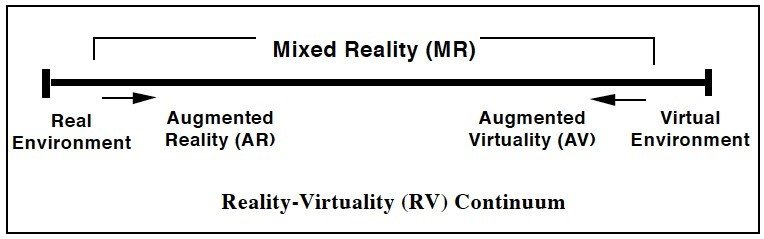
\includegraphics[scale=0.5]{pics/reality_virtuality_continuum}
    \caption{Reality Virtuality Continuum}
    \label{fig:reality_virtuality_continuum}
\end{figure}

In dieser Arbeit sprechen wir über die Wirklichkeit welche durch ein head mounted display, oder umgangssprachlich auch eine VR-Brille angezeigt wird.
Somit bezeichnet eine VR Application eine Software, welche in der VR-Brille läuft.

Von diesen VR Applikationen gibt es schon einige.
lt. einer Statistik aus Deutschland aus dem Jahr 2021, bei welcher Personen mit einer VR-Brille oder head mounted display befragt worden sind, wird VR meistens im Bereich Videospiele verwendet.
Details zu dieser Befragung siehe Abb.~\ref{fig:statistic_usage_vr}.

\begin{figure}
    \begin{center}
        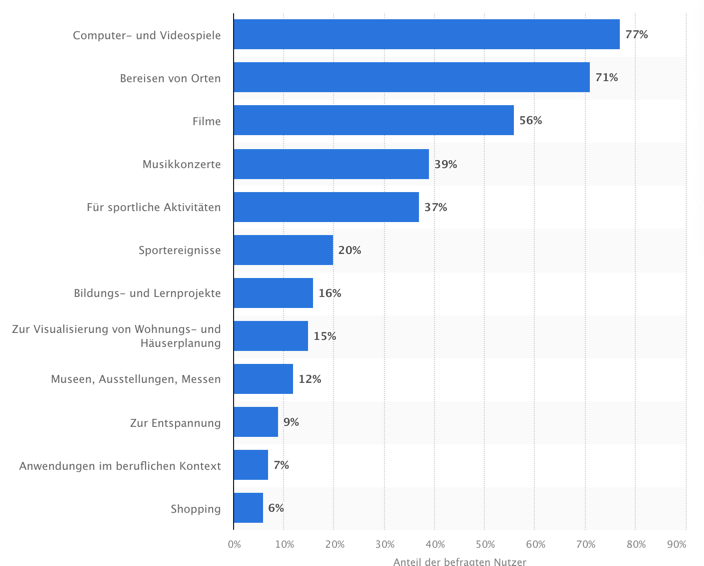
\includegraphics[scale=0.4]{pics/statistic_usage_vr}
    \end{center}
    \caption{Anwendungsgebiete VR~\cite{BITKOM_2021}}
    \label{fig:statistic_usage_vr}
\end{figure}

VR Applikationen haben sich in der Vergangenheit hauptsächlich auf das Tracking des Kopfes konzentriert.
Das Tracken weiterer Körperteile oder ein sogenanntes Full Body Tracking, also das Tracken der Füße, Hände, Hüfte und des Kopfes, war bis vor kurzem ein technisches und vor allem auch ein finanzielles Problem~\cite{PAVEL_NUZHDIN_2020}.

Im Falle der bestehenden Anwendung VR Chat werden zwei Vive Tracker (siehe~\ref{sec:vive-tracker}) verwendet um den linken und den rechten Fuß zu tracken und ein weiterer um die Hüfte zu tracken.
Für die Hände und den Kopf werden jeweils die Controller und das VR Headset (siehe Abschnitt~\ref{sec:vr-headset}) verwebtet.
Somit kann der ganze Körper getrackt werden, da die restlichen positionen berechnetet werden können.
Diese Implementierung kann zum Beispiel bei der Applikation VR Chat gefunden werden (siehe~\cite{VRCHAT_DOCS_2021} oben).
In der Dokumentation wird es auch 6PT oder six-point genannt.
VR Chat bietet auch ein weniger genaues Tracking an welches nur einen Tracker, zwei Controller und das VR Headset verwendet.

Ein weiterer Schritt im Reality-Virtuality Continuum~\cite{MILGRAM_1994} ist die Einbindung realer Gegenstände in die virtuelle Welt.
Man spricht in diesem Fall von Augmented Virtuality.
Dadurch wird der Grad an Immersion (siehe~\cite{EMEST_ADAMS_2004} und~\cite{BJOERK_2003}), also wie real die virtuelle Welt vom Benutzer wahrgenommen wird, erhöht.

\section{Zielsetzung}
\label{sec: objective}
\setauthor{Quirin Ecker}

Das Ziel dieser Arbeit is eine Applikation der Augmented Virtuality.
Im Fall von Beam VR wird ein Holzsparren, welcher in der realen Welt auf dem Boden liegt, in der virtuellen Welt als Balken, der aus einem Wolkenkratzer ragt, wahrgenommen.
% TODO: (Quirin Ecker)(optional) Siehe eine Abbildung von der realen Umgebung und eine von der virtuellen Umgebung
Die Applikation soll einem das Gefühl vermitteln, dass man wirklich auf einem Balken steht, welcher von einem Hochhaus wegsteht.
Der Nutzer soll eine Erhöhung spüren sobald er in der virtuellen Realität auf den Balken steigt.

Das Ziel von Beam VR ist die physische Realität und die virtuelle Realität zu kombinieren.
Ein Balken soll in der physischen Realität und in der virtuellen Realität existieren und die gleiche Position einnehmen.
Auch, wenn man sich in seinem Wohnzimmer oder auch anderswo ohne Gefahren befindet.
Beam VR ist nicht der Erfinder dieses Konzeptes.
Mehr dazu gibt es in der kommenden Umfeldanalyse.

Bei der Auswahl der verwendeten Technologien wurde ausschließlich PC basierte VR Hardware verwendet.
Der Fokus auf diese Form der Technologie war von außen vorgegeben, da der Auftraggeber ausschließlich PC basierte Hardware und keine Spielkonsolen verwendet.
